\documentclass[10pt]{article}
\usepackage[utf8]{inputenc}
\usepackage[T1]{fontenc}
\usepackage[version=4]{mhchem}
\usepackage{stmaryrd}
\usepackage[margin=0.5in, tmargin=1in]{geometry}
\usepackage{xcolor}
\usepackage{graphicx}

\usepackage{fancyhdr}
\pagestyle{fancy}
\fancyhf{}
\fancyhead[L]{Math 1A Spring 2024 Notes}
\fancyhead[R]{Alexis Fernandez}
\renewcommand{\headrulewidth}{0.4pt}

\usepackage{enumitem}
\setlist[enumerate]{leftmargin=*}

\usepackage{amsmath, amsfonts, amssymb}

\author{}
\date{}


\begin{document}

\section*{\centering Note 2 - Types of Functions}

\subsection*{The Types of Functions}
Understanding function types and their rules can help us in finding their domains.
\begin{itemize}
    \item \textbf{Linear}: 
    $$y = {\color{blue}m}x + {\color{red}b}$$
    In the above equation, {\color{blue}$m$} is the {\color{blue}slope} and {\color{red}$b$} is the {\color{red}y-intercept}.
    \begin{figure}[h]
        \centering
        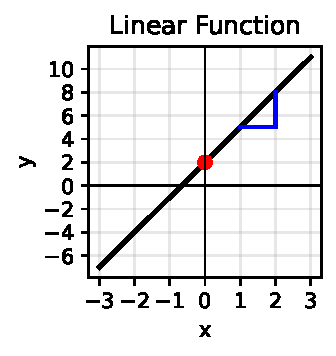
\includegraphics[height=6cm]{../../images/note02/linear.pdf}
    \end{figure} 
    \item \textbf{Polynomial}: 
    $$f(x) = {\color{blue}a}x^{\color{magenta}n}+{\color{blue}b}x^{n-1}+\cdots+{\color{blue}c}x^2+{\color{blue}d}x+{\color{blue}e}$$
    where the coefficients and constant are real numbers, or {\color{blue}$a, b, c, d, e$} $\in \Re$.
    The exponent, {\color{magenta}$n$}, is the degree of the function. \\
    Common types of polynomials are:
    \begin{itemize}[label=$\circ$]
        \item Constant $n=0$
        \item Linear $n=1$
        \item Quadratic $n=2$
        \item Cubic $n=3$
    \end{itemize}
    \item \textbf{Power}: 
    $$f(x) = {\color{blue}k}x^{\color{red}a}$$

    where ${{\color{blue}k}, \color{red}a} \in \Re$ and ${\color{blue}k}, {\color{red}a} \neq 0$. Essentially, a single-term polynomial function where a variable base is raised to  fixed exponent.
    \item \textbf{Rational}: 
    $$f(x) = \dfrac{P(x)}{Q(x)}$$
    where $P(x)$ and $Q(x)$ are polynomial functions.
    \item \textbf{Algebraic}: 
    $$f(x) = ax^n+bx^{n-1}+\cdots+cx^2+dx+e$$
    The set of all real numbers (inputs), {\color{blue}$x$}, for which the function is defined or exists.
    \item \textbf{Trigonometric}: 
    $$f(x) = ax^n+bx^{n-1}+\cdots+cx^2+dx+e$$
    The set of all real numbers (inputs), {\color{blue}$x$}, for which the function is defined or exists.
    \item \textbf{Exponential}: 
    $$f(x) = b^x$$
    The set of all real numbers (inputs), {\color{blue}$x$}, for which the function is defined or exists.
    \item \textbf{Logarithmic}: 
    $$f(x) = \log_{b}x$$
    The set of all real numbers (inputs), {\color{blue}$x$}, for which the function is defined or exists.

\end{itemize}

\end{document}

